\documentclass[a4paper,norsk]{article}
\usepackage{preamble}

\begin{document}
\maketitle
In this project we are going to work with the nonlinear diffusion model

\begin{align}
\varrho u_t = \nabla \cdot (\alpha(u) \nabla u) + f(\textbf{x},t)
\hspace{1cm} \textbf{x} \in \Omega, t \in (0, T]
\end{align}
With $\varrho$ is an constant, and $\alpha(u)$ is a known function of u
.The following initial and boundary condition apply
\begin{align}
u(\textbf{x},0) &= I(x) \hspace{1cm} \textbf{x} \in \Omega, t \in (0, T] \\
\frac{\partial u}{\partial n} &= 0 \hspace{1.5cm} \textbf{x} \in \partial\Omega_D, t \in (0, T]
\end{align}

\section*{Exercise a}
Choosing the Backward Euler discretization, I get the following implicit scheme. 

\begin{align}
\varrho \frac{u^n - u^{n-1}}{\Delta t} = 
\nabla \cdot (\alpha(u^n) \nabla u^n) f(u^n)
\end{align}
Where $u(\textbf{x})^n$ denotes the solution of \textit{u} at timestep \textit{n}
Using the finite element method we want to approximate u in space  
$V = span{\psi_0(x),\psi_1(x),..,\psi(x)_N}$, where $\psi_j$ denotes the basis functions of \textit{V}. To derive a 
variational formulation of the initial condition, we simply multiply or initial condition function \textit{I(\textbf{x})} with a testfunction from our space \textit{V}, and integrate over our domain $\Omega$
\begin{align}
\int_\Omega I v \hspace{2mm}dx = (I,v) = 0
\end{align}
For notation, we redefine the current and last timestep $u^n, u^{n-1}$, as ${u}$ and $u^{(1)}$.
Regarding the total system we first reorganize our equation as
\begin{align}
u - \frac{\Delta t}{\varrho} \nabla \cdot (\alpha(u)\nabla u ) =
u^{(1)} + \frac{\Delta t}{\varrho} f(\textbf{x}, t)
\end{align}
We now multiply the system with a testfunction v, $\forall v \in V$ and integrate over the domain $\Omega$. Utilizing Green's first identity, we can rewrite the second term as follows.

\begin{align}
-\int_\Omega \nabla \cdot (\alpha(u) \nabla u) v \hspace{1mm} dx = 
\int_\Omega (\alpha(u) \nabla u) \cdot \nabla v \hspace{1mm} dx 
- \int_\Omega \alpha(u) \frac{\partial u}{\partial n} v \hspace{1mm}ds
\end{align} 
Using the boundarycondition, the boundary integral equals zero. Using the inner product notation as (,\hspace{2mm}), we can write the variationalform as follows

\begin{align}
(u, v) + \frac{\Delta t}{\varrho}(\alpha(u) \nabla u),\nabla v) = 
(u^{(1)},v) + \frac{\Delta t}{\varrho} (f(\textbf{x}, t), v)
\end{align}

\section*{Exercise b}
To solve the implicit system we will implement Picard iteration, using the recently computed \textit{u} in the $\alpha(u)$ function. Our goal is to linearize the system. Letting $u^{n,k}$ be the calculated \textit{u} after \textit{k} Picard iterations. Our system yields

\begin{align}
u^{n,k+1} - \frac{\Delta t}{\varrho} \nabla \cdot (\alpha(u^{n,k}\nabla u^{n,k+1} ) =
u^{(1)} + \frac{\Delta t}{\varrho} f(\textbf{x}, t)
\end{align}
Our initial guess $u^{n,k=0}$ which starts the iteration, will be the previous time step which we denote as $u^-$. Replacing 
$u^{n,k+1}$ as \textit{u} which is the unknown we want to solve for, 
and using the variational form we can write the system in a simble form
%u - \frac{\Delta t}{\varrho} \nabla \cdot (\alpha(u^-\nabla u ) =
%u^{(1)} + \frac{\Delta t}{\varrho} f(\textbf{x}, t)
\begin{align}
(u, v) + \frac{\Delta t}{\varrho}(\alpha(u^-) \nabla u),\nabla v) = 
(u^{(1)},v) + \frac{\Delta t}{\varrho} (f(\textbf{x}, t), v)
\end{align}

\section*{Exercise c}
\begin{lstlisting}[style=codesnippet]
    def Piccard(self, iterations, getstep = None):
    	#Define Functionspace
        mesh = self.mesh

    	V = FunctionSpace(mesh, 'CG', 1); self.V = V
    	u = TrialFunction(V)
    	v = TestFunction(V)

		#Initial Condition    	
    	u0 = self.u0
    	u_1 = interpolate(u0, V)
    	#Define variatonal problem
        dt = self.dt; q = self.q; T = self.T
    	a = u*v*dx + dt/q*self.alpha_func(u_1)*inner(nabla_grad(u), nabla_grad(v))*dx
    	L = (u_1 + dt/q*self.f_func() )*v*dx
    	A = assemble(a)
    	u = Function(V)
       Nt = int(round(T/dt)+1)
        E_list = np.zeros(Nt+1)
    	error = 1
    	k = 0
 
        for i in range(1, Nt+1):
            #self.f_func().t = i*dt 
            self.f.t = i*dt
            while error > 1E-5 and k < iterations:  
                b = assemble(L)
                solve(A, u.vector(), b)
                k += 1
                u_1.assign(u) 
                error = errornorm(u,u_1)

            if getstep == i*dt:
                u0.t = i*dt
                ue = interpolate(u0, V)
                e = ue.vector().array() - \
                    u_1.vector().array()
                E = np.sqrt(np.sum(e*e)/u_1.vector().array().size)
                self.u = u_1
                return E
        self.u = u 
        return u
\end{lstlisting}

\section*{Exercise d}
For our first verification of the FEniCS implementation, we will try to reproduce a constant solution $u(\textbf{x},t) = C$ where C is some arbitary constant. Implementing this solution into our equation, we observe the following relations

\begin{itemize}
\item \hspace{1mm}$u_t = 0$ \hspace{5mm} implies $\varrho$ can be chosen arbitary
\item $\nabla u = 0$ \hspace{3mm} implies $\alpha$ can be chosen arbitary
\item $f(\textbf{x},t) = 0$
\item $I(\textbf{x}) = C$
\end{itemize}

\begin{lstlisting}[style=codesnippet]
    for i in range(1,3): #Testing P1 and P2 elements
                while dim <= 3: #Increasing dimention of solutionspace
                    sol.define_mesh(Dim[dim-1])
                    u = self.sol.Piccard(1, P_element = i)
                    u_vector = u.vector().array()
                    #u_vector[0]-1E-5 because of small round off errors
                    test = all(x == u_vector[0]-1E-5 for x in u_vector)
                    assert(test == True) #Test if all values are equal
                    dim += 1
                dim = 1
\end{lstlisting}
For constant solution the assert test will not be raised, which is my output in my coderun.

\section*{Exercise e}
We know want to take a step furhter, and try to reproduce an analytical solution. We will assume the following
\begin{itemize}
\item $\alpha(u) = 1$
\item $f(\textbf{x},t) = 0$
\item $\Omega = [0,1] \times [0,1]$ with P1 elements
\item $I(\textbf{x}) = cos(\pi x) $ 
\end{itemize}
These assumptions will result in the manufactured solution $u(x,y,t) = e^{-\pi^2 t} cos(\pi x)$ \\
Error in space is $\mathcal{O}(\Delta x^2) + (\Delta y^2)$, while for time $\mathcal{O}(\Delta t^p)$. \\
We can then write a model for the error such that \\
$E = K_t\Delta t^p + K_x \Delta x^2 + K_y \Delta y^2 = Kh$, where $h = \Delta t^p = \Delta x^2 = \Delta y^2$ \\
By reducing h, we are to show that $\frac{E}{h}$ remains approximately constant as h is redfined. By dividing h by 2 for each run I get the following result. 

\begin{lstlisting}[style = terminal]
E/h = 1.0827 for t=0.01000 seconds
E/h = 1.0861 for t=0.00500 seconds
E/h = 1.0901 for t=0.00250 seconds
E/h = 1.0838 for t=0.00125 seconds
E/h = 1.0849 for t=0.00063 seconds
\end{lstlisting} 
We observe that this ratio remains approximately constant.

\section*{Exercise f}
In this exercise we will test our solver with a manufactured solution. Restricting us to one space dimension, define 
$\alpha(u) = 1 + u^2$ we choose u(x,t) such that
\begin{align}
u(x,t) = t \int_0^x q(1-q)\hspace{1mm}dq = tx^2\big(\frac{1}{2} - \frac{x}{3} \big)
\end{align}
Using the presented sympycode to calculated f, we compare the numerical solution with the manufactured solution.

\begin{figure}[h!]
  \centering
    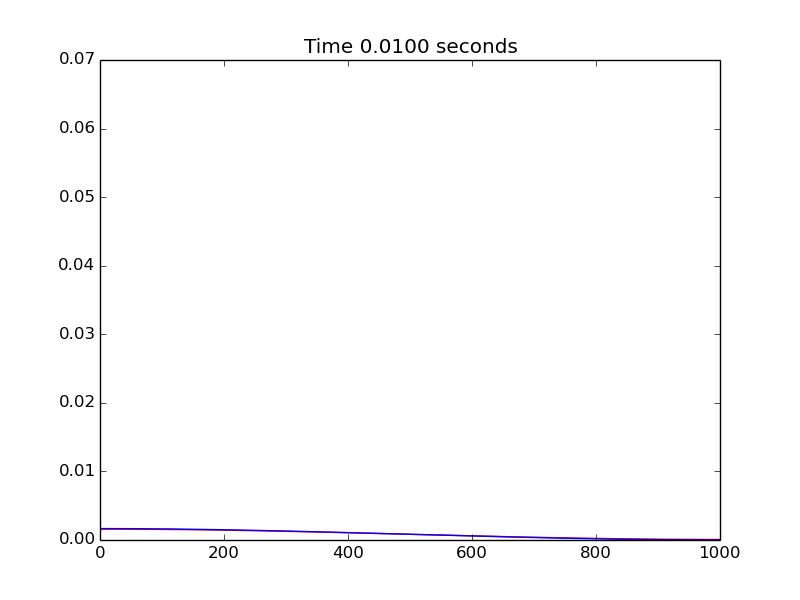
\includegraphics[width=0.4\textwidth]{framea.png}
    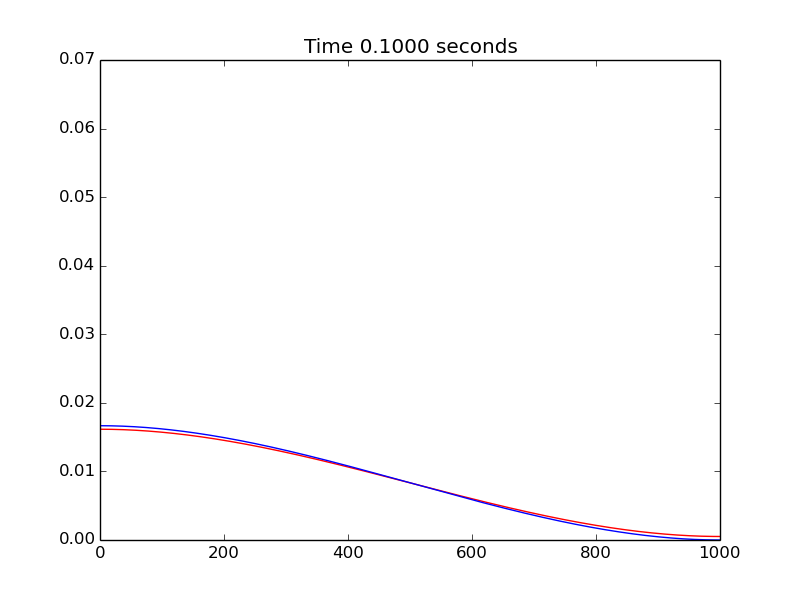
\includegraphics[width=0.4\textwidth]{frameb.png}
\end{figure}

\begin{figure}[h!]
    \centering
    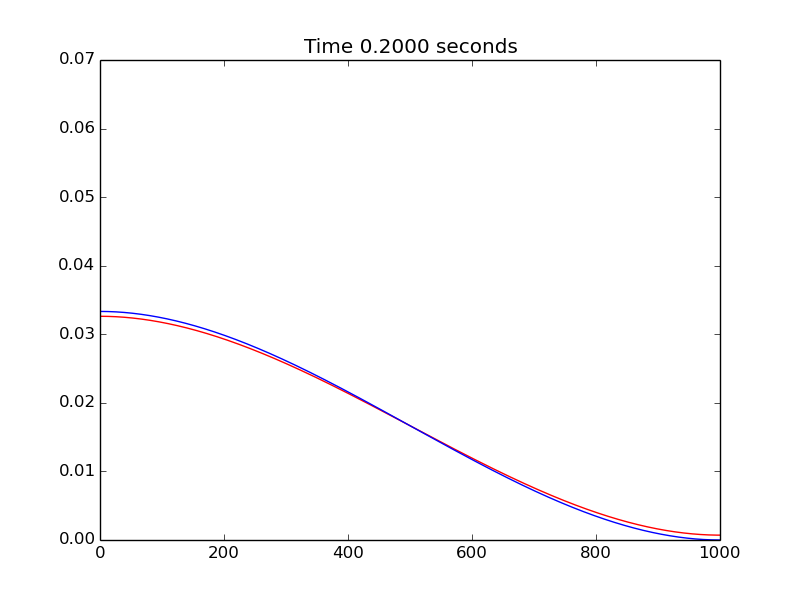
\includegraphics[width=0.4\textwidth]{framec.png}
    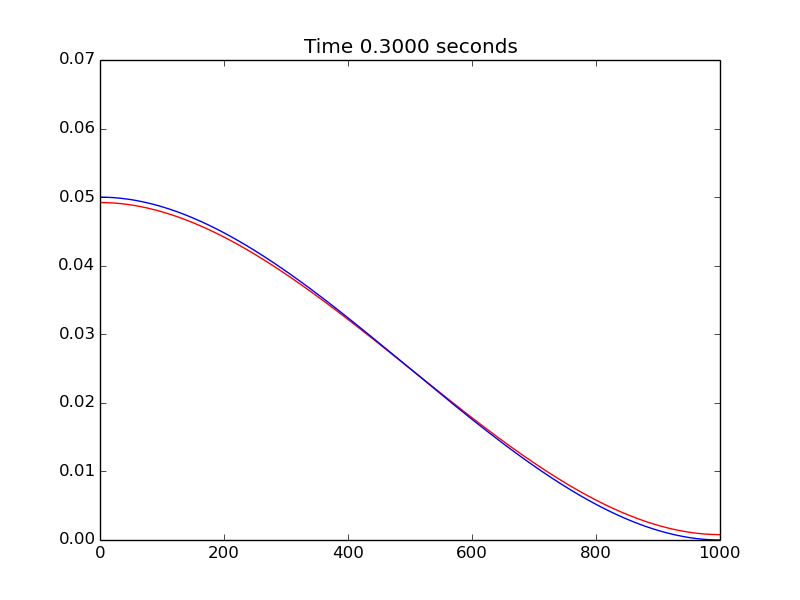
\includegraphics[width=0.4\textwidth]{framed.png}
\end{figure}
Which are some satisfying results.

\section*{Exercise g}
Errors contributing to errors in the numerical calculations.
\begin{itemize}
\item Numerical Integration in the variational form
\item Choosing a finite number of functions in our functionspace to represent the solution.
\item The values of dt and dx, chosen to high
\item Choosing only one Piccard iteration
\end{itemize}

\section*{Exercise h}
Using the presented sympy code we will try to eliminate the error due to a single Picard iteration. This by
producing a manufactured solution for $\alpha(u^{(1)})$. We keep the solution from exercise \textit{f}, and 
$\alpha(u) = 1 + u^2 $. Using the relation $h=\Delta t = \Delta x^2$ we will make a convergence test by assuming 
$E \sim h^r$, showing that r tends to converge to 1. My numerical solver produce the following

\begin{lstlisting}[style = terminal]
 1.00082805  1.00553296  1.00521814  1.00479102  1.0026296]
\end{lstlisting}

\newpage
\section*{Exercise i}
Finally we will simulate the nonlinear diffusion equation of a Gaussian function. 
\begin{align}
I(x,y) = exp(-\frac{1}{2\sigma^2} (x^2+y^2) ) 
\hspace{5mm}
(x,y) \in \Omega = [0,1] \times [0,1]
\end{align}
For my solution I chose $\sigma = 0.09, \beta = 100.0$,
Check out the gaussian.gif file, to see animation of the solution. 

\end{document}